\documentclass[12pt, a4paper]{ctexart}
\usepackage{geometry}
\geometry{left=2.5cm, right=2.5cm, top=3cm, bottom=3cm}
\usepackage{listings}
\usepackage{graphicx}
\usepackage{xcolor}
\usepackage{tikz}
\usetikzlibrary{positioning, fit}

% Code snippet settings
\lstset{
    basicstyle=\ttfamily\small,
    frame=single,
    framesep=5pt,
    xleftmargin=10pt,
    xrightmargin=10pt,
    keywordstyle=\color{blue},
    commentstyle=\color{gray},
    breaklines=true
}

\begin{document}

% 封面
\begin{titlepage}
    \centering
    \vspace*{5cm}
    {\Huge\bfseries 实验报告\par}
    \vspace{2cm}
    {\Large 课程：数字逻辑与计算机组成实验\par}
    \vspace{1cm}
    {\Large 实验二：加法器与 ALU\par}
    \vspace{4cm}
    {\large 姓名：\underline{\makebox[4cm]{郑袭明}}\par}
    \vspace{1cm}
    {\large 学号：\underline{\makebox[4cm]{251502027}}\par}
    \vspace{1cm}
    {\large 日期：\today\par}
\end{titlepage}

\tableofcontents
\newpage

\section{实验目的}
本实验旨在设计并实现一个能够完成带符号补码数的加减法、取反、
与、或、异或及比较大小等8种功能的4位 ALU，
并在 FPGA 开发板上完成硬件验证与结果的数码管显示。

\section{环境配置}
本次及以后实验没有使用课上常用的 Vivado GUI 进行操作，
而是使用了 \texttt{Makefile} 结合 \texttt{.tcl} 脚本的编译方式，
可以使用 \texttt{make} 一键完成编译和烧录等操作。

\begin{lstlisting}[language=make]
VIVADO = vivado -mode batch -source
TCL_SCRIPT = run.tcl
BITSTREAM = ./build/top.bit

all: $(BITSTREAM)

$(BITSTREAM): ./*.v ./*.xdc $(TCL_SCRIPT)
    mkdir -p build
    $(VIVADO) $(TCL_SCRIPT)

prog: $(BITSTREAM)
    $(VIVADO) download.tcl

clean:
    rm -rf build/ .Xil/ *.log *.jou *.html *.xml 

.PHONY: all prog clean
\end{lstlisting}

\section{实验原理与设计}

\begin{figure}[h]
    \centering
    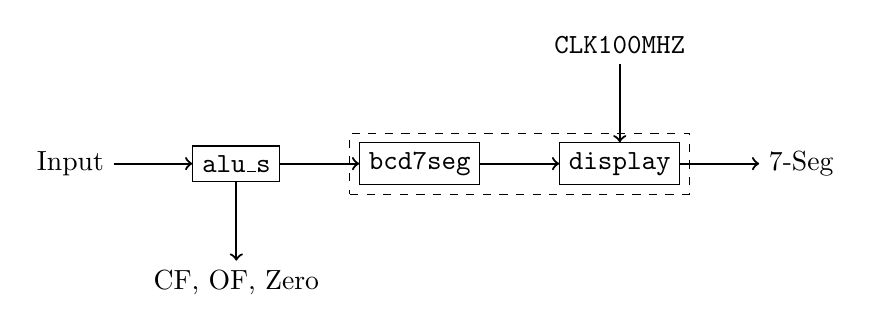
\begin{tikzpicture}
        \node (alu) [draw] {\texttt{alu\_s}};
        \node (bcd) [draw, right=of alu] {\texttt{bcd7seg}};
        \node (disp) [draw, right=of bcd] {\texttt{display}};
        \node (seg) [draw, dashed, fit=(bcd) (disp)] {};
        \node (in) [left=of alu] {Input};
        \node (clk) [above=of disp] {\texttt{CLK100MHZ}};
        \node (out) [right=of disp] {7-Seg};
        \node (pm) [below=of alu] {CF, OF, Zero};
        \draw [->, thick] (in) -- (alu);
        \draw [->, thick] (alu) -- (bcd);
        \draw [->, thick] (bcd) -- (disp);
        \draw [->, thick] (clk) -- (disp);
        \draw [->, thick] (alu) -- (pm);
        \draw [->, thick] (disp) -- (out);
    \end{tikzpicture}
    \caption{系统整体结构图}
    \label{fig:sys}
\end{figure}

实验主要由两个模块组成，分别是 ALU 模块和数码管显示模块。

\begin{itemize}
    \item ALU 模块：减法的进位使用 ARM 的标准，与 x86 的标准相反。
    \item 数码管显示：轮流显示八个数码管的当前值，
    截取 17 位时钟计数器的最高三位作为当前显示的数码管的索引。
    \begin{lstlisting}[language=Verilog]
reg [16:0] counter;
reg [ 2:0] current;

always @(posedge clk) begin
    counter <= counter + 1;
    current <= counter[16:14];
end

always @(*) begin
    an = 8'b11111111;
    an[current] = 1'b0;
end
    \end{lstlisting}
\end{itemize}

\section{实验总结与反思}

Vivado GUI 模式下创建的工程包含大量杂乱的文件，
并且难以传输、难以管理、难以进行 Git 版本控制，
所以我使用了基于 \texttt{Makefile} 结合 \texttt{.tcl} 脚本的编译方式，
使用其他编辑器进行开发，相比直接使用 Vivado GUI 体验大大提升，
且可以满足我的现实条件（Vivado 仅安装在寝室的台式机上，
日常开发使用 MacBook）。唯一的缺点是，没有办法直接在编辑器中进行仿真和调试，
需要切换到 Vivado GUI 才行。

我感觉 Verilog 的语法很丰富，比如使用 \texttt{\$signed(A)}
对 \texttt{A} 进行有符号数处理，这比直接用位运算比较更为方便。
最开始我还是很不熟悉的，比如我不太理解 \texttt{assign} 和在
\texttt{always @(*)} 块里面赋值的区别；现在对 Verilog
这个语言和其内在的逻辑有了进一步的了解，但应该还是不太够，
我还需要更近一步的学习，尤其是后续时序逻辑方面的内容。

\end{document}